%% Copernicus Publications Manuscript Preparation Template for LaTeX Submissions
%% ---------------------------------
%% This template should be used for copernicus.cls
%% The class file and some style files are bundled in the Copernicus Latex Package, which can be downloaded from the different journal webpages.
%% For further assistance please contact Copernicus Publications at: production@copernicus.org
%% https://publications.copernicus.org/for_authors/manuscript_preparation.html


%% Please use the following documentclass and journal abbreviations for discussion papers and final revised papers.


%% 2-column papers and discussion papers
\documentclass[essd, classical]{copernicus}

%% Journal abbreviations (please use the same for discussion papers and final revised papers)

% Archives Animal Breeding (aab)
% Atmospheric Chemistry and Physics (acp)
% Advances in Geosciences (adgeo)
% Advances in Statistical Climatology, Meteorology and Oceanography (ascmo)
% Annales Geophysicae (angeo)
% ASTRA Proceedings (ap)
% Atmospheric Measurement Techniques (amt)
% Advances in Radio Science (ars)
% Advances in Science and Research (asr)
% Biogeosciences (bg)
% Climate of the Past (cp)
% Drinking Water Engineering and Science (dwes)
% Earth System Dynamics (esd)
% Earth Surface Dynamics (esurf)
% Earth System Science Data (essd)
% Fossil Record (fr)
% Geographica Helvetica (gh)
% Geoscientific Instrumentation, Methods and Data Systems (gi)
% Geoscientific Model Development (gmd)
% Hydrology and Earth System Sciences (hess)
% History of Geo- and Space Sciences (hgss)
% Journal of Micropalaeontology (jm)
% Journal of Sensors and Sensor Systems (jsss)
% Mechanical Sciences (ms)
% Natural Hazards and Earth System Sciences (nhess)
% Nonlinear Processes in Geophysics (npg)
% Ocean Science (os)
% Proceedings of the International Association of Hydrological Sciences (piahs)
% Primate Biology (pb)
% Scientific Drilling (sd)
% SOIL (soil)
% Solid Earth (se)
% The Cryosphere (tc)
% Web Ecology (we)
% Wind Energy Science (wes)


%% \usepackage commands included in the copernicus.cls:
%\usepackage[german, english]{babel}
\usepackage{tabularx}
%\usepackage{cancel}
%\usepackage{multirow}
\usepackage{supertabular}
%\usepackage{algorithmic}
%\usepackage{algorithm}
%\usepackage{amsthm}
%\usepackage{float}
%\usepackage{subfig}
%\usepackage{rotating}

%% My packages
\usepackage{amssymb} %symbole de maths
\usepackage{amsmath} %idem
\usepackage{longtable}
\setlength{\LTleft}{-5cm plus 1 fill}
\setlength{\LTright}{-5cm plus 1 fill}
%% New commands
\newcommand{\logit}{\text{logit}}
\newcommand{\bs}[1]{\boldsymbol{#1}}
\newcommand{\R}{\textnormal{\sffamily{\bfseries{R}}}}
\newcommand{\pkg}[1]{{\fontseries{b}\selectfont #1}}

\begin{document}

\title{Combining global tree cover loss data with historical national
  forest-cover maps to look at six decades of deforestation and forest
  fragmentation in Madagascar}


% \Author[affil]{given_name}{surname}

\Author[1, 2, 3]{Ghislain}{Vieilledent}
\Author[4]{Clovis}{Grinand}
\Author[4]{Fety A.}{Rakotomalala}
\Author[5]{Rija}{Ranaivosoa}
\Author[5]{Jean-Roger}{Rakotoarijaona}
\Author[6, 7]{Thomas F.}{Allnutt}
\Author[1]{Frédéric}{Achard}

\affil[1]{Joint Research Center of the European Commission, Bio-economy Unit, I-21027 Ispra (VA), ITALY}
\affil[2]{Cirad, UPR Forêts et Sociétés, F-34398 Montpellier, FRANCE}
\affil[3]{Forêts et Sociétés, Univ. Montpellier, Cirad, Montpellier, FRANCE}
\affil[4]{ETC Terra, F-75020 Paris, FRANCE}
\affil[5]{Office National pour l'Environnement, 101 Antananarivo, MADAGASCAR}
\affil[6]{Wildlife Conservation Society, 101 Antananarivo, MADAGASCAR}
\affil[7]{GreenInfo Network, Oakland, California, USA}

%% The [] brackets identify the author with the corresponding affiliation. 1, 2, 3, etc. should be inserted.

\runningtitle{Six decades of deforestation in Madagascar}

\runningauthor{G. Vieilledent}

\correspondence{Ghislain Vieilledent (ghislain.vieilledent@cirad.fr)}

\received{}
\pubdiscuss{} %% only important for two-stage journals
\revised{}
\accepted{}
\published{}

%% These dates will be inserted by Copernicus Publications during the typesetting process.


\firstpage{1}
\maketitle

\begin{abstract}

  The island of Madagascar has an unparalleled biodiversity, mainly
  located in the tropical forests of the island, which is highly
  threatened by anthropogenic deforestation. Scattered forest maps
  from past studies at national level with substantial gaps (due to
  presence of cloud cover on satellite imagery) prevent the analysis
  of long-term deforestation trends in Madagascar. In this study, we
  propose a new approach combining historical (1953-2000) national
  forest-cover maps with recent (2001-2014) global annual tree cover
  loss data to look at six decades (1953-2014) of deforestation and
  forest fragmentation in Madagascar. We produced new forest-cover
  maps at 30~m resolution over the full territory of Madagascar for
  the year 1990, and annually from 2000 to 2014. We estimated that
  Madagascar has lost 44\% of its natural forest cover over the period
  1953-2014 (including 37\% over the period 1973-2014). Natural
  forests cover 8.9 Mha in 2014 (15\% of the national territory) which
  are divided into 4.4 Mha (50\%) of moist forests, 2.6 Mha (29\%) of
  dry forests, 1.7 Mha of spiny forests (19\%) and 177,000 ha (2\%) of
  mangroves. Since 2005, the annual deforestation rate has
  progressively increased in Madagascar to reach 99,000 ha/yr during
  2010-2014 (corresponding to a rate of 1.1\%/yr). This increase is
  probably due to rapid population growth (close to 3\%/yr) and to
  poor law enforcement in the country. Around half of the forest
  (46\%) is now located at less than 100~m from the forest
  edge. Accurate forest-cover change maps can be used to assess the
  effectiveness of past and current conservation programs and
  implement new strategies for the future. In particular, forest maps
  and estimates can be used in the REDD+ framework which aims at
  ``Reducing Emissions from Deforestation and Forest Degradation'' and
  for optimizing the current protected area network.
  
\end{abstract}


\copyrightstatement{The article is distributed under the Creative Commons Attribution 4.0 License.}


\section{Introduction}
\label{introduction}

Separated from the African continent and the Indian plate about 165
and 88 million years ago respectively \citep{Ali2008}, the flora and
fauna of Madagascar followed its own evolutionary path. Isolation
combined with a high number of micro-habitats \citep{Pearson2009} has
led to Madagascar's exceptional biodiversity both in term of number of
species and endemism in many taxonomic groups \citep{Crottini2012,
  Goodman2005}. Most of the biodiversity in Madagascar is
concentrated in the tropical forests of the island which can be
divided into four types: the moist forest in the East, the dry forest
in the West, the spiny forest in the South and the mangroves on the
West coast \citep{Vieilledent2016}. This unparalleled biodiversity is
severely threatened by deforestation \citep{Harper2007,
  Vieilledent2013} associated with human activities such as slash-and-burn
agriculture and pasture \citep{Scales2011}. Tropical forests in
Madagascar also store a large amount of carbon \citep{Vieilledent2016}
and high rates of deforestation in Madagascar are responsible for
large CO$_2$ emissions in the atmosphere
\citep{Achard2014}. Deforestation threatens species survival by
directly reducing their available habitat \citep{Brooks2002,
  Tidd2001}. Forest fragmentation can also lead to species extinction
by isolating populations from each other and creating forest patches
too small to maintain viable populations
\citep{Saunders1991}. Fragmentation also increases forest edge where
ecological conditions (such as air temperature, light intensity and
air moisture) can be dramatically modified, with consequences on the
abundance and distribution of species \citep{Murcia1995}. Forest
fragmentation can also have substantial effects on forest carbon
storage capacity, as carbon stocks are much lower at the forest edge
than under a closed canopy \citep{Brinck2017}. Moreover, forest
carbon stocks vary spatially due to climate or soil factors
\citep{Saatchi2011, Vieilledent2016}. As a consequence, accurate and
spatially explicit maps of forest-cover and forest-cover change are
necessary to monitor biodiversity loss and carbon emissions from
deforestation and forest fragmentation, assess the efficiency of
present conservation strategies \citep{Eklund2016}, and implement new
strategies for the future \citep{Vieilledent2013,
  Vieilledent2016}. Simple time-series of forest-cover estimates, such
as those provided by the FAO Forest Resource Assessment report
\citep{Keenan2015} are not sufficient.

Unfortunately, accurate and exhaustive forest-cover maps are not
available for Madagascar for the last fifteen years (2000-2015).
\citet{Harper2007} produced maps of forest cover and forest cover
changes over Madagascar for the years \emph{c.}~1953, \emph{c.}~1973,
1990 and 2000. The \emph{c.}~1953 forest map was derived from the
visual interpretation of aerial photography at coarse scale
(1/1,000,000). Forest maps for the years \emph{c.}~1973, 1990, and
2000 were obtained from supervised classification of Landsat satellite
images at 60~m resolution (for the year 1973) or 30~m resolution (for
years 1990 and 2000) and can be used to derive more accurate estimates
of forest cover (89.5\% accuracy reported for the forest/non-forest
map of year 2000). Nonetheless, maps provided by \citet{Harper2007}
are not exhaustive (due to the presence of clouds in the satellite
imagery), e.g.~11 244~km2 are mapped as unknown cover type for the
year 2000. Using a similar supervised classification approach as in
\citet{Harper2007}, more recent maps have been produced for the
periods 2000-2005-2010 by national institutions, with the technical
support of international environmental NGOs \citep{MEFT2009,
  ONE2013}. Another set of recent forest-cover maps using an advanced
statistical tool for classification, the Random Forest classifier
\citep{Grinand2013, Rakotomalala2015}, was produced for the periods
2005-2010-2013 \citep{ONE2015}. However, these maps are either too old
to give recent estimates of deforestation \citep{MEFT2009, ONE2013},
include large areas of missing information due to images with high
percentage of cloud cover \citep{ONE2013}, or show large
mis-classification in specific areas, especially in the dry and spiny
forest domain for which the spectral answer has a strong seasonal
behavior due to the deciduousness of such forests (overall accuracy is
lower than 0.8 for the dry and spiny forests for the maps produced by
\citet{ONE2015}). Moreover, the production of such forest maps from a
supervised classification approach requires significant resources,
especially regarding the image selection step (required to minimize
cloud cover) and the training step (visual interpretation of a large
number of polygons needed to train the classification algorithm)
\citep{Rakotomalala2015}. Most of this work of image selection and
visual interpretation would need to be repeated to produce new forest
maps in the future using a similar approach.

Global forest or tree cover products have also been published recently
and can be tested at the national scale for
Madagascar. \citet{Kim2014} produced a global forest-cover change map
from 1990 to 2000 (derived from Landsat imagery). This product was
updated to cover the period 1975-2005
(\url{http://glcf.umd.edu/data/landsatFCC/}) but forest-cover maps
after 2005 were not produced. Moreover, the approach used in
\citet{Kim2014} did not accurately map the forests in the dry and
spiny ecosystems of Madagascar (see Fig. 8 in \citet{Kim2014}).
\citet{Hansen2013} mapped tree cover percentage, annual tree cover
loss and gain from 2000 to 2012 at global scale at 30 m
resolution. This product has since been updated and is now available
up to the year 2014 \citep{Hansen2013}. To map forest cover from the
\citet{Hansen2013} product, a tree cover threshold must be selected
(that defines forest cover). Selecting such a threshold is not
straightforward as the accuracy of the global tree cover map strongly
varies between forest types, and is substantially lower for dry
forests than for moist forests \citep{Bastin2017}. Moreover, the
\citet{Hansen2013} product does not provide information on
land-use. In particular the global tree cover map does not separate
tree plantations such as oil palm or eucalyptus plantations from
natural forests \citep{Tropek2014}. Thus, the global tree cover map
from \citet{Hansen2013} cannot be used alone to produce a map of
forest cover \citep{Tyukavina2017}.

In this study, we present a simple approach which combines the maps
from \citet{Harper2007} and products from \citet{Hansen2013} to derive
annual wall-to-wall forest-cover change maps over the period 2000-2014
for Madagascar. We use the forest-cover map provided by
\citet{Harper2007} for the year 2000 (defining the land-use) with the
tree cover loss product provided by \citet{Hansen2013} that we apply
only inside forest areas identified by \citet{Harper2007}. Similar to
the approach of \citet{Harper2007}, we also assess trends in
deforestation rates and forest fragmentation from \emph{c.} 1953 to 2014. The
approach described in this study can help assess the effectiveness of
current conservation strategies, and assist the implementation of
future strategies. Our approach could be easily extended to other
tropical countries that have at least one forest-cover map between
2000 and 2014. This approach can easily be repeated in the future when
tree cover loss products will be updated.

\section{Materials and Methods}
\label{materials-and-methods}

\subsection{Creation of new forest-cover maps of Madagascar from
1953 to 2014}

We produced annual forest/non-forest maps at 30~m resolution for the
full territory of Madagascar for the period 2000-2014 by combining the
forest map of year 2000 from \citet{Harper2007}, and the tree cover
percentage and annual tree cover loss maps over the period 2000-2014
from \citet{Hansen2013}. The 2000 Harper's forest map includes 208,000
ha of unclassified areas due to the presence of clouds on satellite
images, mostly (88\%) within the moist forest domain which covered
4.17 Mha in total in 2000. To provide a label (forest or non-forest)
to these unclassified pixels, we used the 2000 tree cover percentage
map of \citet{Hansen2013} by selecting a threshold of 75\% tree cover
to define forest cover as recommended by other studies for the moist
domain \citep{Achard2014, Aleman2017}. To do so, the Hansen's 2000
tree cover map was resampled on the same grid as the original Harper's
map at 30~m resolution using a bilinear interpolation. We thus obtained
a forest-cover map for the year 2000 covering the full territory of
Madagascar. We then combined this forest-cover map of the year 2000
with the annual tree cover loss maps from 2001 to 2014 provided by
\citet{Hansen2013} to create annual forest-cover maps from 2001 to
2014 at 30~m resolution. To do so, Hansen's tree cover loss maps were
resampled on the same grid as the original Harper's map at 30~m
resolution using a nearest-neighbor interpolation. We also completed
the Harper's forest map of year 1990 by filling unclassified areas
(due to the presence of clouds on satellite images) using our
forest-cover map of year 2000. To do so, we assumed that if forest was
present in 2000, the pixel was also forested in 1990. The remaining
unclassified pixels were limited to a relatively small total area of
\emph{c.} 8,000 ha. We labeled these residual pixels as non-forest, as
for the year 2000. Similarly we completed the Harper's forest map of
year 1973 by filling unclassified areas using our forest-cover map of
the year 1990 assuming that if forest was present in 1990, it was also
present in 1973. Contrary to the year 1990, the remaining unclassified
pixels for year 1973 corresponded to a significant total area of 3.3
million ha. We also reprojected the forest-cover map of year 1953 to a
common projection in order to compare the forest-cover area in 1953
with forest-cover areas at the following dates. This map was produced
by scanning a paper map derived from aerial photos, and thus could not
be perfectly aligned with the other maps produced through digital
processing of satellite imagery \citep{Harper2007}. Finally for all
forest-cover maps from 1973, the isolated single non-forest pixels
(i.e.~fully surrounded by forest pixels) were removed, assuming that
single non-forest pixels inside a forest patch were not corresponding
to deforestation (they might correspond to selective logging
activities). This allowed us to avoid counting very small scale events
(\textless 0.1 ha, such as selective logging) as forest
fragmentation. All the resulting maps are freely available at
\url{https://bioscenemada.cirad.fr/forestmaps}.

\subsection{Computing forest-cover areas and deforestation
rates}

From these new forest-cover maps, we calculated the total forest-cover
area for seven available years (1953-1973-1990-2000-2005-2010-2014),
and the annual deforested area and annual deforestation rate for the
corresponding six time periods between 1953 and 2014. The annual
deforestation rates were calculated using Eq.~\ref{eq:theta}
\citep{Puyravaud2003, Vieilledent2013}:

\begin{equation}
  \label{eq:theta}
  \theta = 100 \times [1-(1-(F_{t_2}-F_{t_1})/F_{t_1})^{(1/(t_2-t_1))}
\end{equation}

In Eq.~\ref{eq:theta}, $\theta$ is the annual deforestation rate (in \%/yr),
$F_{t_2}$ and $F_{t_1}$ are the forest cover free of clouds at both
dates $t_2$ and $t_1$, and $t_2-t_1$ is the time-interval (in
years) between the two dates.

Because of the large unclassified area (3.3 million ha) in 1973, the
annual deforestation areas and rates for the two periods 1953-1973 and
1973-1990 are only partial estimates computed on the basis of the
available forest extent. Area and rate estimates are produced at the
national scale and for the four forest ecosystems present in
Madagascar: moist forest in the East, dry forest in the West, spiny
forest in the South, and mangroves on the Western coast
(Fig.~\ref{fig:ecoregion}). To define the forest domains, we used a
map from the MEFT (\emph{``Ministère de l'Environnement et des Forêts
  à Madagascar''}) with the boundaries of the four ecoregions in
Madagascar. Ecoregions were defined on the basis of climatic and
vegetation criteria using the climate classification by
\citet{Cornet1974} and the vegetation classification from the 1996
IEFN national forest inventory \citep{IEFN1996}. Because mangrove
forests are highly dynamic ecosystems that can expand or contract on
decadal scales depending on changes in environmental factors
\citep{Armitage2015}, a fixed delimitation of the mangrove ecoregion
on six decades might not be fully appropriate. As a consequence, our
estimates of the forest-cover and deforestation rates for mangroves in
Madagascar must be considered with this limitation.

\begin{figure}[h]
  \centering
    
    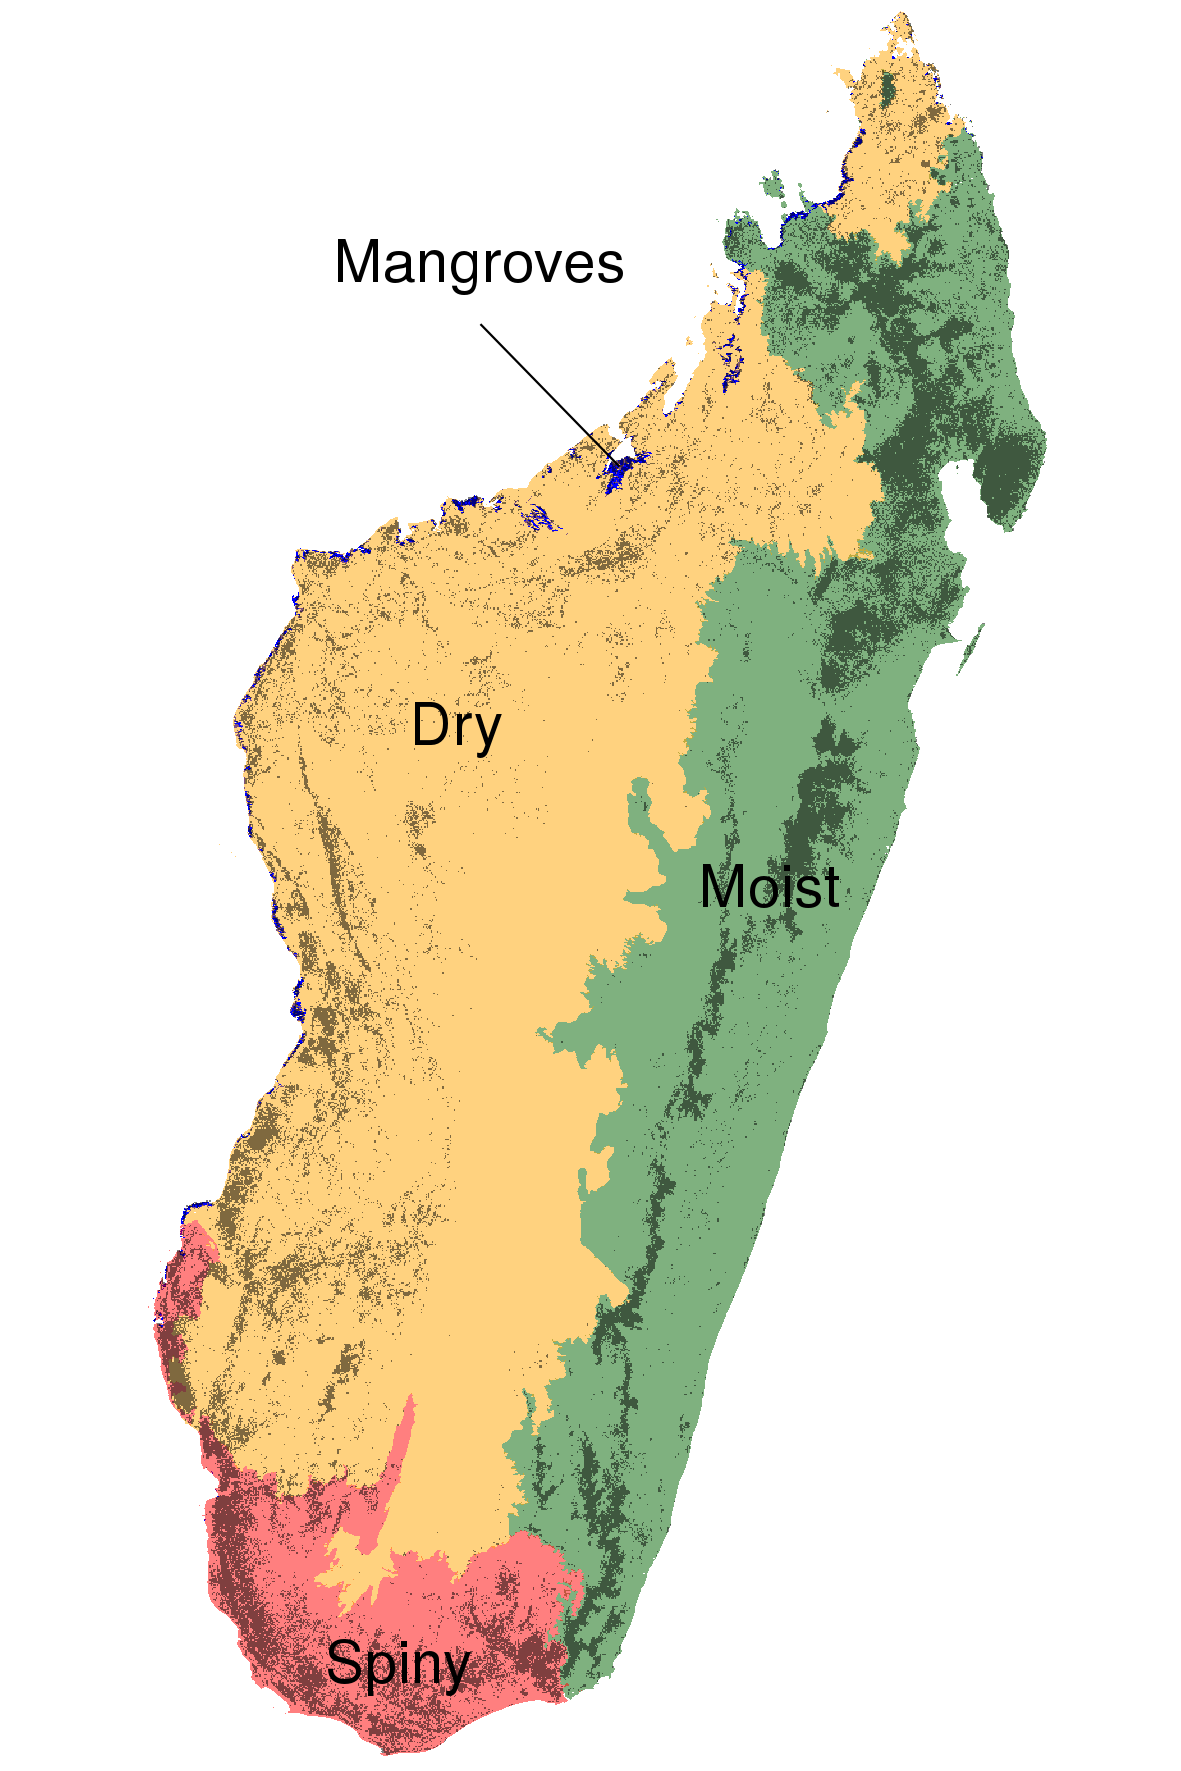
\includegraphics[width=8.3cm]{ecoregion.png}
    
    \caption{\textbf{Ecoregions and forest types in Madagascar.}
      Madagascar can be divided into four climatic ecoregions with four forest
      types: the moist forest in the East (green), the dry forest in the West
      (orange), the spiny forest in the South (red), and the mangroves on the
      West coast (blue). Ecoregions were defined following climatic
      \citep{Cornet1974} and vegetation \citep{IEFN1996} criteria. The dark
      grey areas represent the remaining natural forest cover for the year
      2014.}

    \label{fig:ecoregion}
    
\end{figure}

\subsection{Comparing our forest-cover and deforestation rate
estimates with previous studies}

We compared our estimates of forest-cover and deforestation rates with
estimates from the three existing studies at the national scale for
Madagascar: (i) \citep{Harper2007}, (ii) \citep{MEFT2009} and (iii)
\citep{ONE2015}. \citet{Harper2007} provides forest-cover and
deforestation estimates for the periods
c. 1953-c. 1973-1990-2000. MEFT, USAID, and CI (2009) provides
estimates for the periods 1990-2000-2005 and ONE, DGF, MNP, WCS, and
Etc Terra (2015) provides estimates for the periods 2005-2010-2013. To
compare our forest-cover and deforestation estimates over the same
time periods, we consider an additional time-period in our study
(2010-2013) by creating an extra forest-cover map for the year
2013. We computed the Pearson's correlation coefficient and the root
mean square error (RMSE) between our forest-cover estimates and
forest-cover estimates from previous studies for all the dates and
forest types (including also the total forest cover estimates). For
previous studies, the computation of annual deforestation rates (in
\%/yr) is not always detailed and might slightly differ from one study
to another \citep[see][]{Puyravaud2003}. \citet{Harper2007} also
provide total deforested areas for the two periods 1973-1990 and
1990-2000. We converted these values into annual deforested area
estimates. When annual deforested areas were not reported (for
1953-1973 in \citet{Harper2007} and in \citet{MEFT2009} and
\citet{ONE2015}), we computed them from the forest-cover estimates in
each study. These estimates cannot be corrected from the potential
bias due to the presence of residual clouds. Forest-cover and
deforestation rates were then compared between all studies for the
whole of Madagascar and the four ecoregions. The same ecoregion
boundaries as in our study were used in \citet{ONE2015} but this was
not the case for \citet{Harper2007} and \citet{MEFT2009}, which can
explain a part of the differences between the estimates.

\subsection{Fragmentation}

We also conducted an analysis of changes in forest fragmentation for
the years 1953, 1973, 1990, 2000, 2005, 2010 and 2014 at 30~m
resolution. We applied the method developed by \citet{Riitters2000}
which uses a moving window to characterize the fragmentation around
each forested pixel. Computations were done using the function
\texttt{r.forestfrag} of the GRASS GIS software
\citep{Neteler2008}. Six categories of fragmentation were identified
from the amount of forest and its occurrence as adjacent forest
pixels: ``interior'', ``perforated'', ``edge'', ``transitional'',
``patch'', and ``undetermined''. Previous studies have shown that
micro-habitats were mainly altered within the first 100~m of the
forest edge \citep{Brinck2017, Gibson2013, Murcia1995,
  Broadbent2008}. To characterize fragmentation, we have used a moving
window of 7x7 pixels (4.4~ha). Using this window size, forest edge had
a width of about 90~m \citep{Riitters2000}, which is close to the
value of 100~m and conservative regarding edge effects. The
``interior'' category can be interpreted as the most intact forest
\citep{Potapov2017}. The ``patch'' and ``transitional'' categories
correspond to isolated small forest patches. We reported the area of
forest in each fragmentation category for the six years and analyzed
the dynamics of fragmentation over the six decades. We also computed
the distance to forest edge for all forest pixels for the years 1953,
1973, 1990, 2000, 2005, 2010 and 2014. For that, we used the function
\texttt{gdal\_proximity.py} of the GDAL library
(\url{http://www.gdal.org/}). We computed the mean and 90\% quantiles
(5\% and 95\%) of the distance to forest edge and looked at the
evolution of these values with time.

\begin{figure*}[h]
  \centering
  
  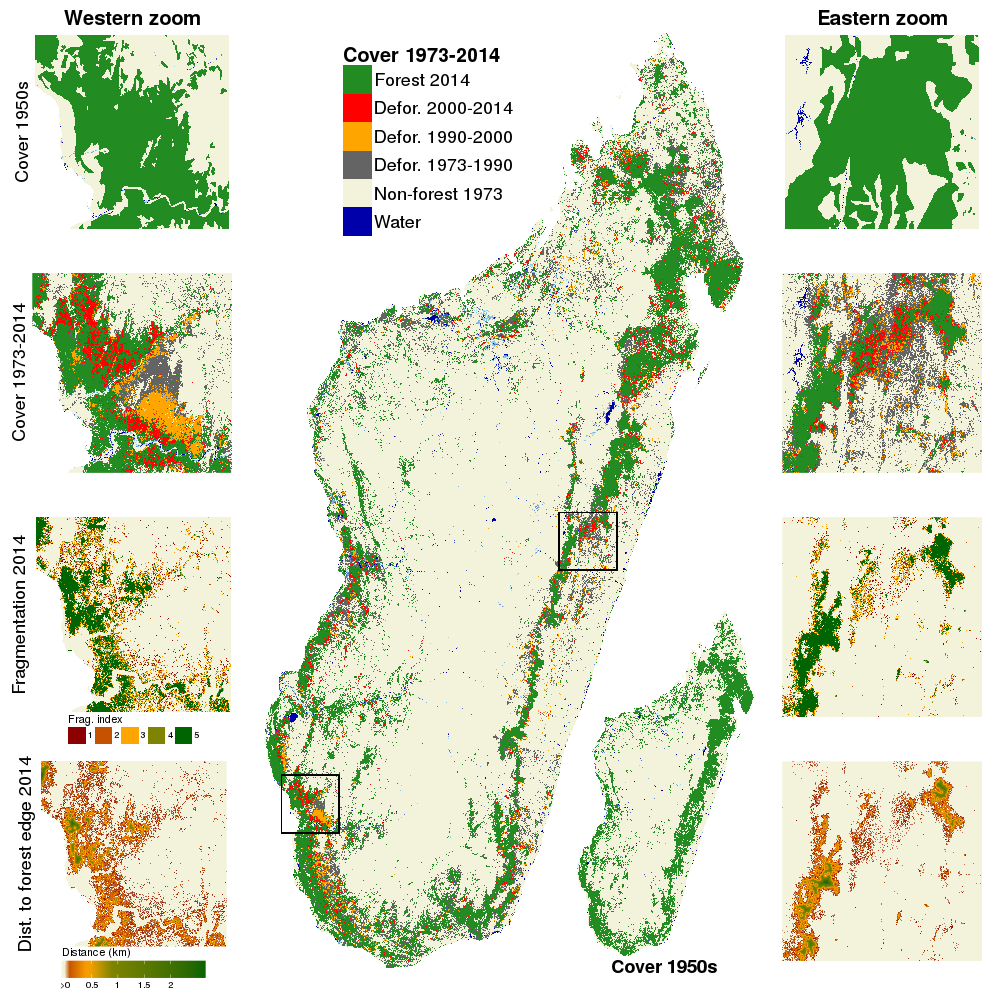
\includegraphics[width=\textwidth]{fig_fcc_highres.png}
  
  \caption{\textbf{Forest-cover change on six decades from 1953
      to 2014 in Madagascar.} Forest cover changes from \emph{c.} 1973 to 2014
    are shown in the main figure, and forest cover in \emph{c.} 1953 is
    shown in the bottom-right inset. Two zooms in the western dry (left
    part) and eastern moist (right part) ecoregions present more detailed
    views of (from top to bottom): forest-cover in 1950s, forest-cover
    change from \emph{c.} 1973 to 2014, forest fragmentation in 2014 and
    distance to forest edge in 2014. Data on water bodies (blue) and water
    seasonality (light blue for seasonal water to dark blue for permanent
    water) has been extracted from \citet{Pekel2016}.}

  \label{fig:fcc}

\end{figure*}

\section{Results}
\label{results}

\subsection{Dynamics of forest cover and deforestation
intensity}

Natural forests in Madagascar covered 16.0 Mha in 1953, about 27\% of
the national territory of 587,041 km2. In 2014, the forest cover
dropped to 8.9 Mha, corresponding to about 15\% of the national
territory (Fig.~\ref{fig:fcc} and
Tab.~\ref{tab:forest_cover}). Madagascar has lost 44\% and 37\% of its
natural forests between 1953 and 2014, and between 1973 and 2014
respectively (Fig.~\ref{fig:fcc} and Tab.~\ref{tab:forest_cover}). In
2014 the remaining 8.9 Mha of natural forest were distributed as follow: 4.4
Mha of moist forest (50\% of total forest cover), 2.6 Mha of dry
forest (29\%), 1.7 Mha of spiny forest (19\%) and 0.18 Mha (2\%) of
mangrove forest (Fig.~\ref{fig:ecoregion} and
Tab.~\ref{tab:comp_forest}). Regarding the deforestation trend, we
observed a progressive decrease of the deforestation rate after 1990
from 205,000 ha/yr (1.6\%/yr) over the period 1973-1990 to 42,000
ha/yr (0.4\%/yr) over the period 2000-2005
(Tab.~\ref{tab:forest_cover}). Then from 2005, the deforestation rate
has progressively increased and has more than doubled over the period
2010-2014 (99,000 ha/yr, 1.1\%/yr) compared to 2000-2005
(Tab.~\ref{tab:forest_cover}). The deforestation trend characterized
by a progressive decrease of the deforestation rate over the period
1990-2005 and a progressive increase of the deforestation after 2005
is valid for all four ecoregions (Tab.~\ref{tab:comp_defor}), with the
exception of the spiny forest domain for which the deforestation rate
during the period 2010-2013 was lower than during 2005-2010
(Tab.~\ref{tab:comp_defor}).

\begin{table}[h]
  
  \caption{\textbf{Evolution of forest cover and deforestation
      rates from 1953 to 2014 in Madagascar}.}
  \label{tab:forest_cover}
  
  \begin{tabular}{@{}lrrrr@{}}
    \tophline
    Year & Forest & Unmapped & Annual defor. & Rate \\
    & (Kha) & (Kha) & (Kha/yr) & (\%/yr) \\
    \middlehline
    1953 & 15,968 & 0 & - & - \\
    1973 & 14,243 & 3,317 & 86 & 0.6 \\
    1990 & 10,762 & 0 & 205 & 1.6 \\
    2000 & 9,879 & 0 & 88 & 0.8 \\
    2005 & 9,668 & 0 & 42 & 0.4 \\
    2010 & 9,320 & 0 & 70 & 0.7 \\
    2014 & 8,925 & 0 & 99 & 1.1 \\
    \bottomhline
  \end{tabular}

  \belowtable{Areas are provided in thousands of hectares
    (Kha). Forest map for the year 1973 has 3.3 Mha of unclassified
    areas due to the presence of clouds on satellite images. As a
    consequence, partial deforestation rates for the periods 1953-1973
    and 1973-1990 are computed based on the available forest
    extent. The last two columns indicate the annual deforested areas
    and annual deforestation rates on the previous time-period
    (e.g.~1953-1973 for year 1973, 1973-1990 for year 1990, etc.).}

\end{table}

\subsection{Comparison with previous forest-cover change studies
in Madagascar}

Forest-cover maps provided by previous studies over Madagascar were
not exhaustive (unclassified areas) due to the presence of clouds on
satellite images used to produce such maps. In \citet{Harper2007}, the
maps of years 1990 and 2000 include 0.5 and 1.12 Mha of unknown cover
type respectively. Proportions of unclassified areas are not reported
in the two other existing studies at the national level by
\citet{MEFT2009} and \citet{ONE2015}. With our approach, we produced
wall to wall forest-cover change maps from 1990 to 2014 for the full
territory of Madagascar (Tab.~\ref{tab:forest_cover}). This allowed us
to produce more robust estimates of forest-cover and deforestation
rates over this period. Our forest-cover estimates over the period
1953-2013 (considering forest cover estimates at national level and by
ecoregions for all the available dates) were well correlated
(Pearson's correlation coefficient $=$ 0.99) to estimates from the
three previous studies (Tab.~\ref{tab:comp_forest}) with a RMSE of
300,000 ha (6\% of the mean forest cover of 4.8 Mha when considering
all dates and forest types together). These small differences can be
partly attributed to differences in ecoregion boundaries. Despite
significant differences in deforestation estimates
(Tab.~\ref{tab:comp_defor}), a similar deforestation trend was
observed across studies with a decrease of deforestation rates over
the period 1990-2005, followed by a progressive increase of the
deforestation after 2005.

\begin{table*}[h]

  \caption{\textbf{Comparing Madagascar forest-cover estimates (in Kha)
      with previous studies on the period 1953-2014}.}
  \label{tab:comp_forest}

  \begin{tabular}{@{}llrrrrrrrr@{}}
    \tophline
    Forest type & Source & 1953 & 1973 & 1990 & 2000 & 2005 & 2010 & 2013 &
                                                                            2014 \\
    \middlehline
    Total & Harper2007 & 15,996 & 14,173 & 10,606 & 8,982 & - & - & - & - \\
          & MEFT2009 & - & - & 10,650 & 9,678 & 9,413 & - & - & - \\
                & ONE2015 & - & - & - & - & 9,451 & 8,977 & 8,486 & - \\
                & this study & 15,968 & 14,243 & 10,762 & 9,879 & 9,668 & 9,320 & 9,051
                                                                          & 8,925 \\
    Moist & Harper2007 & 8,766 & 6,876 & 5,234 & 4,167 & - & - & - &
                                                                     - \\
                & MEFT2009 & - & - & 5,271 & 4,788 & 4,700 & - & - & - \\
                & ONE2015 & - & - & - & - & 4,556 & 4,457 & 4,345 & - \\
                & this study & 8,578 & 6,990 & 5,270 & 4,872 & 4,768 & 4,633 & 4,470 &
                                                                                       4,410 \\
    Dry & Harper2007 & 4,252 & 4,028 & 2,712 & 2,457 & - & - & - &
                                                                   - \\
                & MEFT2009 & - & - & 3,321 & 3,085 & 3,028 & - & - & - \\
                & ONE2015 & - & - & - & - & 3,223 & 2,970 & 2,679 & - \\
                & this study & 4,762 & 4,435 & 3,225 & 2,941 & 2,881 & 2,735 & 2,642 &
                                                                                       2,596 \\
    Spiny & Harper2007 & 2,978 & 3,030 & 2,420 & 2,132 & - & - & - &
                                                                     - \\
                & MEFT2009 & - & - & 2,124 & 1,872 & 1,757 & - & - & - \\
                & ONE2015 & - & - & - & - & 1,682 & 1,559 & 1,467 & - \\
                & this study & 2,463 & 2,583 & 2,055 & 1,858 & 1,811 & 1,744 & 1,731 &
                                                                                       1,713 \\
    Mangroves & Harper2007 & - & - & 240 & 226 & - & - & - &
                                                             - \\
                & MEFT2009 & - & - & - & - & - & - & - & - \\
                & ONE2015 & - & - & - & - & 174 & 171 & 170 & - \\
                & this study & 143 & 200 & 181 & 178 & 177 & 177 & 177 &
                                                                         177 \\
    \bottomhline
  \end{tabular}

  \belowtable{We compared our estimates of forest-cover with the
    estimates from three previous studies \citep{Harper2007, MEFT2009,
      ONE2015}. Areas are provided in thousands of hectares (Kha). We
    obtained a Pearson's correlation coefficient of 0.99 between our
    forest-cover estimates and forest-cover estimates from previous
    studies. The increase in mangrove and spiny forest covers from
    \emph{c.} 1953 to \emph{c.} 1973 in \citet{Harper2007} and our
    study is most probably due to differences in forest definition and
    mapping methods between the 1953 aerial-photography derived map
    and the 1973 Landsat image derived map.}

\end{table*}

\begin{table*}[h]

  \caption{\textbf{Comparing Madagascar annual deforestation rates
      with previous studies on the period 1953-2014}.}
  \label{tab:comp_defor}
  
  \begin{tabular}{@{}llrrrrrr@{}}
    \tophline
    Forest type & Source & 1953-1973 & 1973-1990 & 1990-2000 & 2000-2005 &
                                                                           2005-2010 & 2010-2013\\
    \middlehline
    Total & Harper2007 & 91 (0.3) & 200 (1.7) & 81 (0.9) & - & - &
                                                                   - \\
                & MEFT2009 & - & - & 97 (0.8) & 53 (0.5) & - & - \\
                & ONE2015 & - & - & - & - & 95 (1.2) & 164 (1.5) \\
                & this study & 86 (0.6) & 205 (1.6) & 88 (0.9) & 42 (0.4) & 70 (0.7) &
                                                                                       90 (1.0) \\
    Moist & Harper2007 & 94 (0.6) & 87 (1.7) & 32 (0.8) & - & - &
                                                                  - \\
                & MEFT2009 & - & - & 48 (0.8) & 17 (0.4) & - & - \\
                & ONE2015 & - & - & - & - & 20 (0.5) & 37 (0.9) \\
                & this study & 79 (1.0) & 101 (1.6) & 40 (0.8) & 21 (0.4) & 27 (0.6) &
                                                                                       54 (1.2) \\
    Dry & Harper2007 & 11 (0.2) & 77 (1.9) & 20 (0.7) & - & - &
                                                                - \\
                & MEFT2009 & - & - & 24 (0.7) & 11 (0.4) & - & - \\
                & ONE2015 & - & - & - & - & 51 (1.8) & 97 (2.3) \\
                & this study & 16 (0.4) & 71 (1.9) & 28 (0.9) & 12 (0.4) & 29 (1.0) & 31
                                                                                      (1.1) \\
    Spiny & Harper2007 & -3 (-0.1) & 36 (1.2) & 28 (1.2) & - & - &
                                                                   - \\
                & MEFT2009 & - & - & 25 (1.2) & 23 (1.2) & - & - \\
                & ONE2015 & - & - & - & - & 25 (1.7) & 31 (1.7) \\
                & this study & -6 (-0.2) & 31 (1.3) & 20 (1.0) & 9 (0.5) & 13 (0.7) & 4
                                                                                      (0.3) \\
    Mangroves & Harper2007 & - & - & 1 (0.2) & - & - & - \\
                & MEFT2009 & - & - & - & - & - & - \\
                & ONE2015 & - & - & - & - & 0 (0.3) & 0 (0.2) \\
                & this study & -3 (-1.7) & 1 (0.6) & 0 (0.2) & 0 (0.0) & 0 (0.0) & 0
                                                                                   (0.0) \\
    \bottomhline
  \end{tabular}

  \belowtable{Annual deforestated areas (in Kha/yr) and annual
    deforestation rates (second number in parenthesis, in \%/yr) are
    provided. For deforestation rates in \%/yr, exact same numbers as
    in scientific articles and reports from previous studies
    \citep{Harper2007, MEFT2009, ONE2015} have been reported. The way
    annual deforestation rates in \%/yr have been computed in these
    previous studies can slightly differ from one study to another, but
    estimates always correct for the potential presences of clouds on
    satellite images and unclassified areas on forest maps. Annual
    deforested areas in Kha/yr have been recomputed from forest-cover
    estimates in Tab.~\ref{tab:comp_forest} (except for
    \citet{Harper2007} for the periods 1973-1990 and 1990-2000 for
    which annual deforested areas in Kha/yr were derived from numbers
    reported in the original publication, see methods) and do not
    correct for the potential presence of clouds.}

\end{table*}

\subsection{Evolution of forest fragmentation with time}

In parallel to the dynamics of deforestation, forest fragmentation has
progressively increased since 1953 in Madagascar. We observed a
continuous decrease of the mean distance to forest edge from 1953 to
2014 in Madagascar. The mean distance to forest edge has decreased to
\emph{c.} 300~m in 2014 while it was previously \emph{c.} 1.5~km in 1973
(Fig.~\ref{fig:dist_edge}). Moreover, a large proportion (73\%) of
the forest was located at a distance greater than 100 m in 1973, while
almost half of the forest (46\%) was at a distance lower than 100 m
from forest edge in 2014 (Fig.~\ref{fig:dist_edge}). The percentage of
forest that can be considered intact in Madagascar has continuously
decreased since 1953. The percentage of forest belonging to the
``interior'' category (most intact forests) has fallen from 68\% in
1973 to 50\% in 2014. In 2014, more than 16\% of the forest belonged
to the ``patch'' and ``transitional'' categories (isolated small
forest patches) compared to 9\% in 1973 (Tab.~\ref{tab:frag}).

\begin{figure}[h]
  \centering
  
  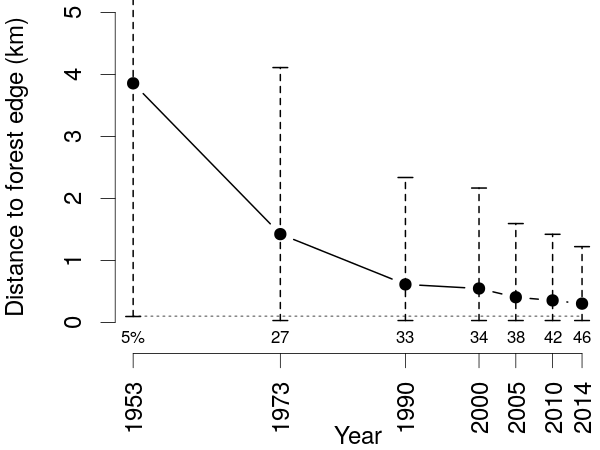
\includegraphics[width=8.3cm]{dist.png}
  
  \caption{\textbf{Evolution of the distance to forest edge from 1953
      to 2014 in Madagascar.} Black dots represent the mean distance
    to forest edge for each year. Vertical dashed segments represent
    the 90\% quantiles (5\% and 95\%) of the distance to forest
    edge. Horizontal dashed grey line indicates a distance to forest
    edge of 100~m.  Numbers at the bottom of each vertical segments are
    the percentage of forest at a distance to forest edge lower than
    100~m for each year.}

  \label{fig:dist_edge}

\end{figure}

\section{Discussion}
\label{discussion}

\subsection{Benefits of the combined use of recent global annual
  tree cover loss data with historical national forest-cover maps}

In this study, we combined recent (2001-2014) global annual tree cover
loss data \citep{Hansen2013} with historical (1953-2000) national
forest-cover maps \citep{Harper2007} to look at six decades
(1953-2014) of deforestation and forest fragmentation in
Madagascar. We produced annual forest-cover maps at 30~m resolution
covering Madagascar for the period 2000 to 2014. Our study extends the
forest-cover monitoring on a six decades period (from 1953 to 2014)
while harmonizing the data from previous studies \citep{Harper2007,
  MEFT2009, ONE2015}. We propose a generic approach to solve the
problem of forest definition which is needed to transform the 2000
global tree cover dataset from \citet{Hansen2013} into a
forest/non-forest map \citep{Tropek2014}. We propose to use a
historical national forest-cover map, based on a national forest
definition, as a forest cover mask. This approach could be easily
extended to other regions or countries for which an accurate
forest-cover map is available at any date within the period 2000-2014,
but preferably at the beginning of the period to profit from the full
record and derive long-term estimates of deforestation. Moreover, this
approach can be repeated in the future if and when the global tree
cover product is updated. We have made the \R{}/GRASS code used for this
study freely available in a GitHub repository (see Data availability
statement) to facilitate application to other study areas or repeat
the analysis in the future for Madagascar.

The accuracy of the derived forest-cover change maps depends directly
on the accuracies of the historical forest-cover maps and the tree
cover loss dataset. Using visual-interpretation of aerial images in
342 areas distributed among all forest types, \citet{Harper2007}
estimated an overall 89.5\% accuracy in identifying forest/non-forest
classes for the year 2000. The accuracy assessment of the tree cover
loss dataset for the tropical biome reported 13\% of false positives
and 16.9\% of false negatives (see Tab. S5 in
\citet{Hansen2013}). These numbers rise at 20.7\% and 20.6\%
respectively for the subtropical biome. In the subtropical biome, the
lower density tree cover canopy makes it difficult to detect change
from tree cover to bare ground. For six countries in Central Africa,
with a majority of moist dense forest, \citet{Verhegghen2016} have
compared deforestation estimates derived from the global tree cover
loss dataset \citep{Hansen2013} with results derived from
semi-automated supervised classification of Landsat satellite images
\citep{Achard2014} and they found a good agreement between the two
sets of estimates. Therefore, our forest-cover change maps after 2000
might be more accurate for the dense moist forest than for the dry and
spiny forest. In another study assessing the accuracy of the tree
cover loss product accross the tropics \citep{Tyukavina2015}, authors
reported 4\% of false positives and 48\% of false negatives in
Sub-Saharian Africa. They showed that 85\% of missing loss occured on
the edges of other loss patches. This means that tree cover loss might
be underestimated in Sub-Saharian Africa, probably due to the
prevalence of small-scale disturbance which is hard to map at 30~m,
but that areas of large-scale deforestation are well identified and
spatial variability of the deforestation is well represented. A proper
accuracy assessment of our forest-cover change maps should be
performed to better estimate the uncertainty surrounding our
forest-cover change estimates in Madagascar from year 2000
\citep{Olofsson2013,Olofsson2014}. Despite this limitation, we have
shown that the deforestation trend we observed for Madagascar, with a
doubling deforestation on the period 2010-2014 compared to 2000-2005,
was consistent with the other studies at the national scale
\citep{ONE2015, MEFT2009}.

Consistent with \citet{Harper2007}, we did not consider potential
forest regrowth in Madagascar (although \citet{Hansen2013} provided a
tree cover gains layer for the period 2001-2013) for several
reasons. First, the tree gain layer of \citet{Hansen2013} includes and
catches more easily tree plantations than natural forest regrowth
\citep{Tropek2014}. Second, there is little evidence of natural forest
regeneration in Madagascar \citep{Grouzis2001, Harper2007}. This can
be explained by several ecological processes following burning
practice such as soil erosion \citep{Grinand2017} and reduced seed
bank due to fire and soil loss \citep{Grouzis2001}. Moreover, in areas
where forest regeneration is ecologically possible, young forest
regrowth are more easily re-burnt for agriculture and pasture. Third,
young secondary forests provide more limited ecosystem services
compared to old-growth natural forests in terms of biodiversity and
carbon storage.

\subsection{Dynamics of forest-cover in Madagascar from 1953 to 2014}

We estimated that natural forests in Madagascar cover 8.9 Mha in 2014
(corresponding to 15\% of the country) and that Madagascar has lost
44\% of its natural forest since 1953 (37\% since 1973). There is
ongoing scientific debate about the extent of the ``original'' forest
cover in Madagascar, and the extent to which humans have altered the
natural forest landscapes since their large-scale settlement around
800 CE \citep{Burns2016, Cox2012}. Early French naturalists stated
that the full island was originally covered by forest
\citep{Humbert1927, Perrier1921}, leading to the common statement that
90\% of the natural forests have disappeared since the arrival of
humans on the island \citep{Kull2000}. More recent studies
counter-balanced that point of view saying that extensive areas of
grassland existed in Madagascar long before human arrival and were
determined by climate, natural grazing and other natural factors
\citep{Vorontsova2017, Virah-Sawmy2009}. Other authors have questioned
the entire narrative of extensive alteration of the landscape by early
human activity which, through legislation, has severe consequences on
local people \citep{Klein2002, Kull2000}. Whatever the original
proportion of natural forests and grasslands in Madagascar, our
results demonstrate that human activities since the 1950s have
profoundly impacted the natural tropical forests and that conservation
and development programs in Madagascar have failed to stop
deforestation in the recent years. Deforestation has strong
consequences on biodiversity and carbon emissions in
Madagascar. Around 90\% of Madagascar's species are forest dependent
\citep{Allnutt2008, Goodman2005} and \citet{Allnutt2008} estimated
that deforestation between 1953 and 2000 led to an extinction of 9\%
of the species. The additional deforestation we observed over the
period 2000-2014 (around 1Mha of natural forest) worsen this
result. Regarding carbon emissions, using the 2010 aboveground forest
carbon map by \citet{Vieilledent2016}, we estimated that deforestation
on the period 2010-2014 has led to 40.2 Mt C of carbon emissions in
the atmosphere (10 Mt C /yr) and that the remaining aboveground forest
carbon stock in 2014 is 832.8 Mt C. Associated to deforestation, we
showed that the remaining forests of Madagascar are highly fragmented
with 46\% of the forest being at less than 100~m of the forest
edge. Small forest fragments do not allow to maintain viable
populations and ``edge effects'' at forest/non-forest interfaces have
impacts on both carbon emissions \citep{Brinck2017} and biodiversity
loss \citep{Gibson2013, Murcia1995}.

\begin{table}[h]

  \caption{\textbf{Evolution of the forest fragmentation from 1953 to 2014
      in Madagascar}.}
  \label{tab:frag}

  \begin{tabular}{@{}lrrrrrr@{}}
    \tophline
    Year & Forest & patch & transit. & edge & perfor. & interior \\
    & (Kha) & (\%) & (\%) & (\%) & (\%) & (\%) \\
    \middlehline
    1953 & 15,963 & 0 & 1 & 4 & 1 & 94 \\
    1973 & 14,228 & 2 & 7 & 20 & 3 & 68 \\
    1990 & 10,750 & 3 & 8 & 21 & 4 & 64 \\
    2000 & 9,866 & 3 & 8 & 22 & 4 & 62 \\
    2005 & 9,660 & 4 & 9 & 23 & 6 & 59 \\
    2010 & 9,307 & 4 & 10 & 23 & 9 & 55 \\
    2014 & 8,911 & 5 & 11 & 23 & 11 & 50 \\
    \bottomhline
  \end{tabular}

  \belowtable{Five categories of fragmentation were identified from
    the amount of forest and its occurrence as adjacent forest pixels:
    ``interior'', ``perforated'', ``edge'', ``transitional'', and
    ``patch'' \citep{Riitters2000}. We used a moving window of 7x7
    pixels (4.4~ha). Using this window size, forest edge had a width
    of about 90~m. The ``interior'' category can be interpreted as the
    most intact forest. The ``patch'' and ``transitional'' categories
    correspond to isolated small forest patches. Forest areas are
    provided in thousands of hectares (Kha).}

\end{table}

\subsection{Deforestation trend and impacts on conservation and
  development policies}

In our study, we have shown that the progressive decrease of the
deforestation rate on the period 1990-2005 was followed by a
continuous increase in the deforestation rate on the period
2005-2014. In particular, we showed that deforestation rate has more
than doubled on the period 2010-2014 compared to 2000-2005. Our
results are confirmed by previous studies \citep{Harper2007, MEFT2009,
  ONE2015} despite differences in the methodologies regarding (i)
forest definition (associated to independent visual interpretations of
observation polygons to train the classifier), (ii) classification
algorithms, (iii) deforestation rate computation method, and (iv)
correction for the presence of clouds. Our deforestation rate
estimates from 1990 to 2014 have been computed from wall to wall maps
at 30~m resolution and can be considered more accurate in comparison
with estimates from these previous studies. Our forest-cover and
deforestation rate estimates can be used as source of information for
the next FAO Forest Resources Assessment \citep{Keenan2015}. Current
rates of deforestation can also be used to build reference scenarios
for deforestation in Madagascar and contribute to the implementation
of deforestation mitigation activities in the framework of REDD+
\citep{Olander2008}.

The increase of deforestation rates after 2005 can be explained by
population growth and political instability in the country. Nearly
90\% of Madagascar's population relies on biomass for their daily
energy needs \citep{Minten2013} and the link between population size
and deforestation has previously been demonstrated in Madagascar
\citep{Vieilledent2013, Gorenflo2011}. With a mean demographic growth
rate of about 2.8\%/yr and a population which has increased from 16 to
24 million people on the period 2000-2015 \citep{UN2015}, the
increasing demand in wood-fuel and space for agriculture is likely to
explain the increase in deforestation rates. The political crisis of
2009 \citep{Ploch2012}, followed by several years of political
instability and weak governance could also explain the increase in the
deforestation rate observed on the period 2005-2014
\citep{Smith2003}. These results show that despite the conservation
policy in Madagascar \citep{Freudenberger2010}, deforestation has
dramatically increased at the national level since 2005. Results of
this study, including recent spatially explicit forest-cover change
maps and forest-cover estimates, should help implement new
conservation strategies to save Madagascar natural tropical forests
and their unique biodiversity.


%% The following commands are for the statements about the availability of data sets and/or software code corresponding to the manuscript.
%% It is strongly recommended to make use of these sections in case data sets and/or software code have been part of your research the article is based on.

%%\codeavailability{TEXT} %% use this section when having only software code available


%%\dataavailability{TEXT} %% use this section when having only data sets available


\codedataavailability{All the data and codes used for this study are
  made publicly available in the \texttt{deforestmap} GitHub
  repository (\url{https://github.com/ghislainv/deforestmap.git}). The
  results are fully reproducible running the \R{} script
  \texttt{deforestmap.R} located inside the \texttt{deforestmap}
  repository.} %% use this section when having data sets and software code available


%\appendix
%\section{}    %% Appendix A

%\subsection{}     %% Appendix A1, A2, etc.


%\noappendix       %% use this to mark the end of the appendix section

%% Regarding figures and tables in appendices, the following two options are possible depending on your general handling of figures and tables in the manuscript environment:

%% Option 1: If you sorted all figures and tables into the sections of the text, please also sort the appendix figures and appendix tables into the respective appendix sections.
%% They will be correctly named automatically.

%% Option 2: If you put all figures after the reference list, please insert appendix tables and figures after the normal tables and figures.
%% To rename them correctly to A1, A2, etc., please add the following commands in front of them:

%\appendixfigures  %% needs to be added in front of appendix figures

%\appendixtables   %% needs to be added in front of appendix tables

%% Please add \clearpage between each table and/or figure. Further guidelines on figures and tables can be found below.

\authorcontribution{All authors conceived the ideas and designed methodology; GV analysed
the data and wrote the \R{}/GRASS script; GV drafted the manuscript. All
authors contributed critically to the drafts and gave final approval for
publication.} %% optional section

\competinginterests{Authors declare that they have no conflict of interest.}
%% this section is mandatory even if you declare that no competing interests are present

%% \disclaimer{TEXT} %% optional section

\begin{acknowledgements}

  Authors thank Jean-François Bastin for useful comments on a previous
  version of the manuscript. This study is part of the Cirad's
  BioSceneMada project (\url{https://bioscenemada.cirad.fr}) and the
  Joint Research Center's ReCaREDD project
  (\url{http://forobs.jrc.ec.europa.eu/recaredd}). The BioSceneMada
  project is funded by FRB (Fondation pour la Recherche sur la
  Biodiversité) and the FFEM (Fond Français pour l'Environnement
  Mondial) under the project agreement AAP-SCEN-2013 I. The ReCaREDD
  project is funded by the European Commission.
  
\end{acknowledgements}

%% REFERENCES

%% The reference list is compiled as follows:

% \begin{thebibliography}{}

% \bibitem[AUTHOR(YEAR)]{LABEL}
% REFERENCE 1

% \bibitem[AUTHOR(YEAR)]{LABEL}
% REFERENCE 2

% \end{thebibliography}

%% Since the Copernicus LaTeX package includes the BibTeX style file copernicus.bst,
%% authors experienced with BibTeX only have to include the following two lines:
%%
\bibliographystyle{copernicus}
\bibliography{biblio}
%%
%% URLs and DOIs can be entered in your BibTeX file as:
%%
%% URL = {http://www.xyz.org/~jones/idx_g.htm}
%% DOI = {10.5194/xyz}


%% LITERATURE CITATIONS
%%
%% command                        & example result
%% \citet{jones90}|               & Jones et al. (1990)
%% \citep{jones90}|               & (Jones et al., 1990)
%% \citep{jones90,jones93}|       & (Jones et al., 1990, 1993)
%% \citep[p.~32]{jones90}|        & (Jones et al., 1990, p.~32)
%% \citep[e.g.,][]{jones90}|      & (e.g., Jones et al., 1990)
%% \citep[e.g.,][p.~32]{jones90}| & (e.g., Jones et al., 1990, p.~32)
%% \citeauthor{jones90}|          & Jones et al.
%% \citeyear{jones90}|            & 1990

%% FIGURES

%% When figures and tables are placed at the end of the MS (article in one-column style), please add \clearpage
%% between bibliography and first table and/or figure as well as between each table and/or figure.

%% ONE-COLUMN FIGURES

%%f
%\begin{figure}[t]
%\includegraphics[width=8.3cm]{FILE NAME}
%\caption{TEXT}
%\end{figure}
%
%%% TWO-COLUMN FIGURES
%
%%f
%\begin{figure*}[t]
%\includegraphics[width=12cm]{FILE NAME}
%\caption{TEXT}
%\end{figure*}
%
%

%%% TABLES
%%%
%%% The different columns must be seperated with a & command and should
%%% end with \\ to identify the column brake.
%
%%% ONE-COLUMN TABLE
%
%%t
%\begin{table}[t]
%\caption{TEXT}
%\begin{tabular}{column = lcr}
%\tophline
%
%\middlehline
%
%\bottomhline
%\end{tabular}
%\belowtable{} % Table Footnotes
%\end{table}

%%% TWO-COLUMN TABLE
%
%%t
%\begin{table*}[t]
%\caption{TEXT}
%\begin{tabular}{column = lcr}
%\tophline
%
%\middlehline
%
%\bottomhline
%\end{tabular}
%\belowtable{} % Table Footnotes
%\end{table*}

%%% MATHEMATICAL EXPRESSIONS
%
%%% All papers typeset by Copernicus Publications follow the math typesetting regulations
%%% given by the IUPAC Green Book (IUPAC: Quantities, Units and Symbols in Physical Chemistry,
%%% 2nd Edn., Blackwell Science, available at: http://old.iupac.org/publications/books/gbook/green_book_2ed.pdf, 1993).
%%%
%%% Physical quantities/variables are typeset in italic font (t for time, T for Temperature)
%%% Indices which are not defined are typeset in italic font (x, y, z, a, b, c)
%%% Items/objects which are defined are typeset in roman font (Car A, Car B)
%%% Descriptions/specifications which are defined by itself are typeset in roman font (abs, rel, ref, tot, net, ice)
%%% Abbreviations from 2 letters are typeset in roman font (RH, LAI)
%%% Vectors are identified in bold italic font using \vec{x}
%%% Matrices are identified in bold roman font
%%% Multiplication signs are typeset using the LaTeX commands \times (for vector products, grids, and exponential notations) or \cdot
%%% The character * should not be applied as mutliplication sign
%
%
%%% EQUATIONS
%
%%% Single-row equation
%
%\begin{equation}
%
%\end{equation}
%
%%% Multiline equation
%
%\begin{align}
%& 3 + 5 = 8\\
%& 3 + 5 = 8\\
%& 3 + 5 = 8
%\end{align}
%
%
%%% MATRICES
%
%\begin{matrix}
%x & y & z\\
%x & y & z\\
%x & y & z\\
%\end{matrix}
%
%
%%% ALGORITHM
%
%\begin{algorithm}
%\caption{?}
%\label{a1}
%\begin{algorithmic}
%?
%\end{algorithmic}
%\end{algorithm}
%
%
%%% CHEMICAL FORMULAS AND REACTIONS
%
%%% For formulas embedded in the text, please use \chem{}
%
%%% The reaction environment creates labels including the letter R, i.e. (R1), (R2), etc.
%
%\begin{reaction}
%%% \rightarrow should be used for normal (one-way) chemical reactions
%%% \rightleftharpoons should be used for equilibria
%%% \leftrightarrow should be used for resonance structures
%\end{reaction}
%
%
%%% PHYSICAL UNITS
%%%
%%% Please use \unit{} and apply the exponential notation


\end{document}
